\section{Geometria}

\questao{(OM$^3$SP 2026 - 1ª Fase) Na última sexta-feira o professor Henry propôs uma aula diferente. Ele levou todos os alunos dos sextos anos da E.M.M.M.S.P. para a serra do Goití para uma aula de asa-delta. Para dar o exemplo de como seria, ele saltou primeiro e, quase chegando no fim do voo, um aluno tirou uma foto do momento. Nesta foto, o mesmo aluno percebeu que ao ligar as extremidades inferiores da asa-delta formaria um triângulo com ângulos gerados nos dois lados da base valendo $30^\circ$. Assim, ao chegar na escola, o aluno imprimiu a foto e com uma caneta vermelha traçou uma reta nas extremidades e formou o triângulo mostrado na imagem a seguir:}
        \begin{figure}[H]
            \centering
            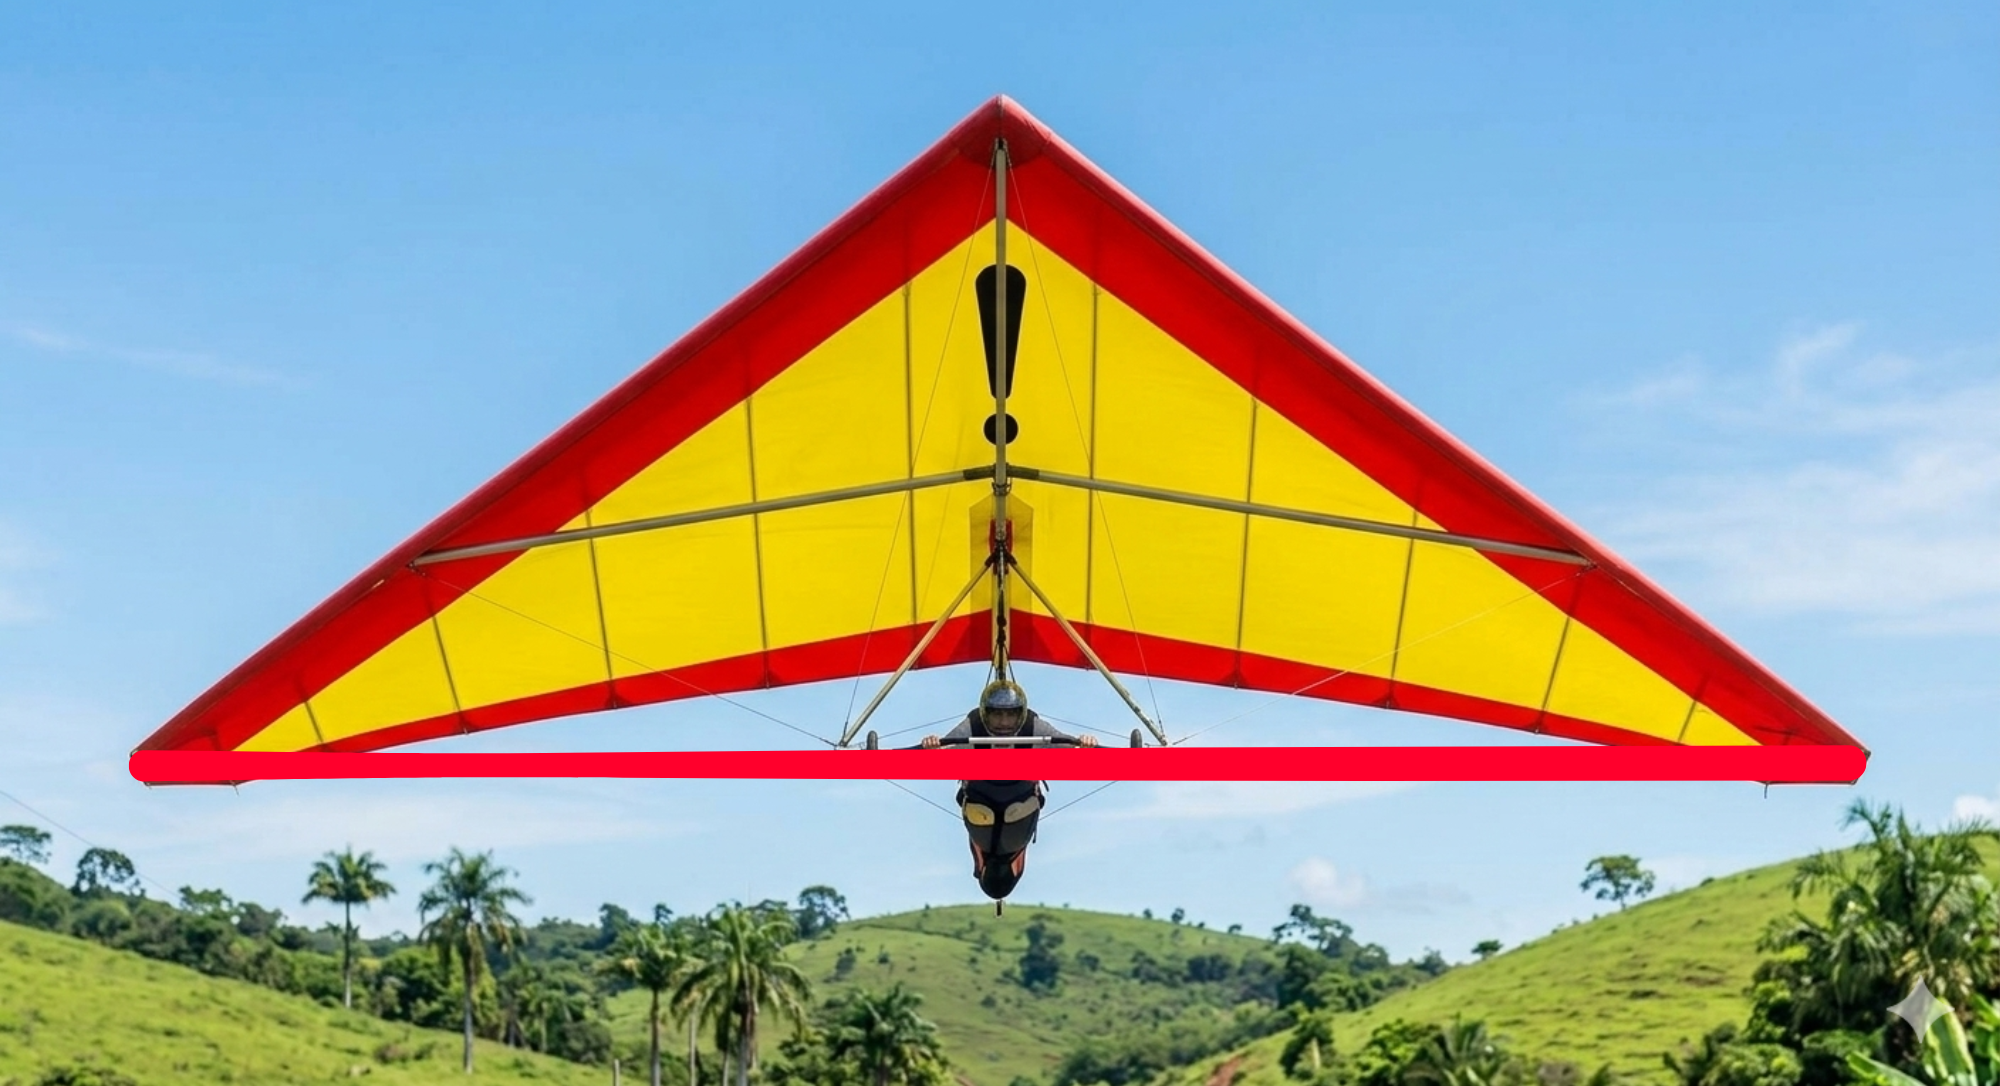
\includegraphics[width=0.5\linewidth]{figuras/6_ano/Asa Delta.png}
        \end{figure}
        Ao ver a foto, o aluno percebeu que poderia classificar esse triângulo. Qual seria a classificação dele considerando os seus ângulos?
         \begin{multicols}{4}
            \begin{enumerate}[label=\alph*)]
                \item retângulo
                \item obtusângulo
                \item acutângulo
                \item minervângulo
            \end{enumerate}
        \end{multicols}

\begin{solucoes}{1}
    \solucao
Nesta questão tem-se um triângulo gerado pela união das duas extremidades inferiores de uma asa-delta. A questão nos informou que os ângulos inferiores gerados possuem $30^\circ$, o que qualifica esse triângulo como isósceles. Como a soma dos ângulos internos de um triângulo vale $180^\circ$, teremos;
        \begin{equation*}
            x+30^\circ+30^\circ =180^\circ
        \end{equation*}
        \begin{equation*}
            x =180^\circ-60^\circ
        \end{equation*}
        \begin{equation*}
            x =120^\circ
        \end{equation*}
        Logo, como temos um ângulo obtuso, o triângulo é obtusângulo.\\
        \textbf{ALTERNATIVA B)}
\end{solucoes}